% CR-I-EIP short paper: when a consumer-metric safety monitor helps, and when
% it hurts. Written on the three sealed families, all three graded FAIL (owner
% directive, 2026-09-06). House style: plain declarative, no em-dashes in prose,
% every number from a committed graded record, negatives disclosed.
% Venue candidate: a mechanistic-interpretability / safety workshop.
\documentclass[11pt]{article}
\usepackage[margin=1in]{geometry}
\usepackage[T1]{fontenc}
\usepackage{lmodern}
\usepackage{amsmath,amssymb}
\usepackage{booktabs}
\usepackage{graphicx}
\graphicspath{{build/}}
\usepackage{url}
\usepackage[hidelinks]{hyperref}

\title{When Reading an Equivariance Monitor's Residual\\ Through the Model Helps, and When It Hurts:\\ Three Sealed Preregistrations and No Forecaster}
\author{Andrew H.\ Bond\\ San Jos\'e State University\\ \texttt{agi.hpc@gmail.com}}
\date{Draft, September 2026}

\begin{document}
\maketitle

\begin{abstract}
An equivariance monitor grades a paraphrase-invariance residual
$e = h_\ell(g x) - \hat\rho_\ell h_\ell(x)$ in raw L2 norm. We ask whether
grading it instead in the downstream model's own read, measured as the model's
output response when $e$ is patched into layer $\ell$, catches more real
behavioral changes at matched flag rates. The effect is real and it is
double-signed. Read through the model, the residual cuts monitor false-clears by
5 to 20 points under backtranslation and 12 to 16 under synonym substitution,
replicated at two model scales, but under paraphrase it inverts, adding 35 to 57
points. This raises the practical question the monitor designer actually faces:
given a transform, will the consumer read help or hurt. We preregistered three
sealed families to answer it, and all three failed their own bars, which we
report as executed. No gate predicted the sign: not the absence of a gate
(family V1), not the equivariance map's own held-out fit (family V2), and not
transform locality, the held-out $R^2$ of the identity map $h_\ell(g x) \approx
h_\ell(x)$ (family V3), which a clean separation on the earlier families had
suggested. The V3 grade is decisive against locality: half-truncation, the most
non-local transform, posts the largest advantage in its family rather than the
predicted none, and interior word-shuffling, which is representationally local,
loses the advantage; the correlation between locality and advantage is
$-0.05$. The phenomenon replicates, but no scalar measured on the representation
forecasts its sign. The design consequence is conservative: a
consumer-metric gate cannot be certified from a calibration-time representation
statistic, and a monitor should keep the raw metric unless the consumer read has
been validated empirically on the transform family it will face.
\end{abstract}

\section{Introduction}

Internal-equivariance monitors gate on $h_\ell(g x) \approx \hat\rho_\ell(g)\,
h_\ell(x)$: a paraphrase $g$ should move a layer's representation the way a
fitted linear map $\hat\rho_\ell$ predicts, and a residual that violates this
flags a possible spec-gaming or drift \cite{ieip2026}. The residual is scored in
raw L2 norm. Observation Theory raises an objection that applies to any such
monitor \cite{turboquant,geoobs}. The
layer's activations have a consumer, the downstream computation, and the norm
that matters is the consumer's read of the residual, not its raw magnitude. A
large residual in a direction the downstream network ignores is a false alarm;
a small residual exactly where the network reads is a false clear, which is the
case the monitor exists to catch.

This paper measures the consumer-read alternative. We grade the residual by its
measured patch-response: inject $e$ at layer $\ell$ and record the model's
output-KL response, the consumer's actual sensitivity to that residual. The
alternative is not uniformly better or worse. It cuts false-clears sharply under
some transforms and inverts under others, so the useful question is not whether
to read through the model but when. We attacked that question the way we would
want a safety claim attacked: three preregistered families, each naming its
cells, pass/fail thresholds, and seeds in version control before any evaluation
data was opened, verdicts committed as executed. All three failed. The failures
are the result. They rule out, in turn, the three variables a designer would
reach for first, and the third rules out a variable that had looked clean on the
first two families. We report what survives: a robust, replicated, double-signed
effect whose sign we cannot yet predict from the representation, and the
conservative rule that this forces.

\section{Related work}

Our instrument is activation patching, the causal-tracing technique that
measures a component's effect on the output by replacing its activation and
reading the change downstream \cite{meng2022,wang2022}. We use it not to localize
a circuit but as the grading norm of a safety monitor: the model's output-KL
response to the injected residual is the consumer's read. The choice of patching
metric is known to change which components look important \cite{zhangnanda2024},
which is why we fix the metric, the flag rate, and the bars in each
preregistration before grading. Reading a representation through a downstream map
is the probing-classifier idea \cite{alain2016}; the consumer read applies it to
a monitor's residual rather than to a labeled concept. The object of study is an
internal-equivariance monitor, which gates on a fitted paraphrase-invariance map
and scores the residual in raw norm \cite{ieip2026}; monitoring and steering a
model by reading its activations is an active safety direction \cite{zou2023}.
The claim that a representation has no single geometry until a consumer reads it,
and the read operator that follows, are developed in the Observation Theory
program and shipped in its public artifacts \cite{turboquant,geoobs}. What is new
here is neither patching nor consumer-relative reading but the measurement of a
monitor built on both, and specifically the sealed negative: the consumer read's
benefit is real and replicated, yet its sign is not forecastable from the three
representation statistics we preregistered. We adopt preregistration in the form
argued for language research by van Miltenburg et al.\ \cite{vanmiltenburg2021},
with pass/fail bars and seeds frozen before grading and failed families reported
as executed. We do not offer a better monitor. We offer the measurement of when
reading a monitor's residual through the model helps, and the evidence that no
representation scalar we tried tells you in advance.

\section{Method}

\textbf{Setup.} An open causal LM (Qwen2.5, 0.5B and 1.5B) reads
Social-Chemistry-101 action texts and their transforms $g x$. For each layer
$\ell$ the whitepaper's ridge estimator fits $\hat\rho_\ell$ on a calibration
split; the residual $e = h_\ell(g x) - \hat\rho_\ell h_\ell(x)$ is injected at
$\ell$ by a last-position activation patch and the metric is the model's
output-KL response to that injection. Ground truth is the model's actual
next-token KL between $x$ and $g x$. A pair is ``behavior-changed'' when that KL
exceeds the calibration 75th percentile. The monitor flags the top quartile by
each metric, matching the flag rates, and the reported quantity is the
false-clear rate, the fraction of behavior-changed pairs not flagged, with the
consumer-read advantage
\[
  \Delta = fc_{\mathrm{raw}} - fc_{\mathrm{true}}.
\]
$\Delta > 0$ means the consumer read clears fewer real changes than raw L2.

\textbf{Discipline.} Each family is a sealed preregistration naming its cells,
bars, seeds, and manipulation checks before any evaluation data is opened, with
a one-day cooling-off between construction and seal. Graded verdicts are
committed exactly as the frozen rules grade them. Sizes were set from measured
memory footprints, not from model weights. All records, seals, per-cell graded
JSONs, and post-mortems are in the campaign repository.

\section{The effect is real, and its sign flips by transform}

Read through the model, the residual is a better monitor under
representation-preserving transforms and a worse one under
representation-relocating transforms. Under backtranslation, the graded cells
cut false-clears by 5 to 20 points at matched flag rates (family V1 cell B,
$-14$ and $-15$ points at 1.5B; family V2 cells D, E, G, from $-5$ to $-20$
points across two scales). Under synonym substitution, family V3 cells H and K
cut them by 12 to 16 points at both scales. The same read inverts under
paraphrase: family V1 cells A and C and family V2 cell F all add 35 to 57 points
of false-clears over raw L2, at both model scales. Injecting a residual that is
dominated by map error probes the model's sensitivity to a direction that is not
the perturbation, while the raw norm degrades gracefully.

Two findings recur under every seal and we state them as robust. The
paraphrase inversion is confirmed at both scales three times over. The
equivariance map's held-out $R^2$ collapses at the final layer in seven of eight
graded runs, from above $0.8$ in calibration to at or below zero, so a monitor
calibrated at the final layer grades against a broken map regardless of which
norm it uses.

\section{Two sealed attempts to gate the effect on map fit both fail}

Family V1 used no gate. It graded FAIL because its bar required a consumer
advantage on every cell and the paraphrase cell inverted. Its post-mortem found
the advantage's magnitude unforecastable from the single-split headroom it had
qualified on.

The natural repair is to gate on the equivariance map's own quality: read
through the model only where $\hat\rho$ generalizes. Family V2 tested this,
gating on the held-out $R^2$ of $\hat\rho$, and graded FAIL, six of eight units
passing and the failure precise. In the deep layers of the 1.5B backtranslation
cells the map's held-out $R^2$ is slightly negative, so the $\hat\rho$-fit gate
calls them out-of-regime, yet the consumer advantage persists there at 9 and 17
points. The advantage does not need a good map. It needs the patched residual to
point roughly along the true perturbation, and map fit is a leaky proxy for
that.

\section{The locality law, preregistered and refuted}

\begin{figure}[t]
  \centering
  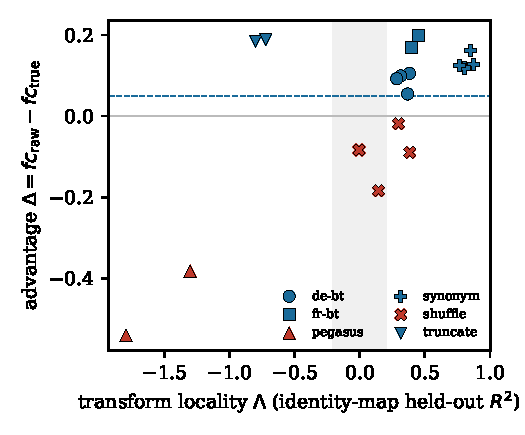
\includegraphics[width=0.8\columnwidth]{fig_delta_lambda.pdf}
  \caption{The consumer-read advantage $\Delta$ against transform locality
  $\Lambda$, the identity-map held-out $R^2$, one point per graded (cell, layer)
  unit across families V2 and V3. Blue points clear more real changes than raw
  L2; red points clear fewer. Locality does not order them: the truncation units
  near $\Lambda = -0.75$ sit as high as the synonym units near $\Lambda = +0.8$,
  and the shuffle units inside the shaded transition band sit below zero. The
  earlier families' clean split was an artifact of the two transforms they
  happened to contain.}
  \label{fig:law}
\end{figure}

On families V1 and V2 a single variable had separated the outcomes with no
overlap: transform locality, how nearly $h_\ell(g x) \approx h_\ell(x)$,
measured as the held-out $R^2$ of the identity map,
\[
  \Lambda_\ell = 1 - \frac{\sum \lVert h_\ell(g x) - h_\ell(x)\rVert^2}
                          {\sum \lVert h_\ell(g x) - \overline{h_\ell(g x)}\rVert^2}.
\]
It requires no map fit. Every backtranslation unit, including the two the
$\hat\rho$-gate got wrong, had $\Lambda$ between $+0.28$ and $+0.45$; both
paraphrase units had $\Lambda$ near $-1.3$ and $-1.8$. The reading was
mechanistic and plausible: where a transform is local, $h_\ell(g x) = h_\ell(x)
+ \delta$ with small $\delta$, so even a noisy $\hat\rho$ leaves the residual
approximately equal to the true perturbation and the consumer read stays
informative; where it relocates the representation, the residual is map error
and the read inverts.

Family V3 preregistered this as a law and tested it on transforms the earlier
families did not contain. It graded five cells on a constructed locality ladder,
from synonym substitution through interior word-shuffling, which is textually
very different yet representationally local, to half-truncation. The sealed
predictions were a threshold law, $\Delta \ge 0.05$ when $\Lambda \ge 0.20$ and
$\Delta \le 0.01$ when $\Lambda \le -0.20$, and a monotonicity, Spearman$(\Lambda,
\Delta) \ge 0.7$ pooled over all units. Both failed, and the failure is not
marginal.

\begin{table}[t]
  \centering
  \small
  \begin{tabular}{llrrl}
    \toprule
    cell (transform) & scale & $\Lambda$ & $\Delta$ & arm result \\
    \midrule
    H (synonym)   & 0.5B & $+0.87,\,+0.85$ & $+0.13,\,+0.16$ & local: pass \\
    K (synonym)   & 1.5B & $+0.80,\,+0.77$ & $+0.12,\,+0.13$ & local: pass \\
    L (shuffle)   & 0.5B & $+0.39,\,+0.30$ & $-0.09,\,-0.02$ & local: \textbf{fail} \\
    I (shuffle)   & 1.5B & $+0.14,\,-0.01$ & $-0.18,\,-0.08$ & band \\
    J (truncate)  & 0.5B & $-0.80,\,-0.72$ & $+0.19,\,+0.19$ & non-local: \textbf{fail} \\
    \bottomrule
  \end{tabular}
  \caption{Family V3, graded (two mid layers per cell). Half-truncation is the
  most non-local transform yet posts the family's largest advantage, where the
  law predicted none; word-shuffling is local yet loses the advantage. Locality
  does not predict the sign.}
  \label{tab:v3}
\end{table}

Table~\ref{tab:v3} shows why. Half-truncation, the most non-local transform in
the study at $\Lambda \approx -0.75$, does not lose the advantage as the law
requires; it posts the largest advantage in the family, about 19 points, where
the bar was $\Delta \le 0.01$. Interior word-shuffling, which is
representationally local, loses the advantage instead of keeping it. Pooled over
all graded units the correlation between locality and advantage is $-0.05$,
against a floor of $0.7$. The consumer advantage appears at both extremes of
locality and vanishes in the middle. The clean separation on families V1 and V2
was a property of the two transforms they happened to contain, not a law.

The V3 grade also corrects the mechanistic reading we drew from V2. Truncation
is more non-local than several backtranslation units and does not invert, so
``non-local implies inversion'' is false. The two transforms that lose the
advantage, shuffle and paraphrase, both rearrange or rewrite tokens while
preserving length and surface plausibility; the two that keep it, backtranslation
or synonym and outright truncation, either barely move the tokens or delete them.
A natural reading is that what governs the sign is whether the decision-relevant
change survives into the patched residual. We tested that reading post-hoc across
all graded units, and it does not forecast the sign either. A directional
survival measure, the cosine between the patched residual and the true
perturbation, is uncorrelated with the advantage (Spearman $0.27$) and does not
separate the advantage units from the inversion units. A stronger measure,
whether patching the residual reproduces the true output change, matches locality
but no more (Spearman $0.59$) and misses on the same cells: truncation has a
large advantage yet low patch fidelity, and shuffling has high patch fidelity yet
none. Four scalars have now failed to forecast the sign: no gate, map fit,
locality, and survival in two forms. The advantage is a tail phenomenon, a
false-clear rate at a matched flag quantile, and no global statistic of the
representation or the patch that we have tried captures it. A forecaster, if one
exists, is future work. This non-forecastability rhymes with an
information-theoretic result in the program's foundational rate--content region
\cite{bondtit}: for a Gaussian source with encoder-observed context, the
operational content is not determined by the consumer's reduced view of the
source. We claim no formal reduction, only that the same shape appears in both
places, a consumer's own view underdetermining the quantity it would need to act
on.

\section{Consequence for monitor design}

Three preregistered predictors of the consumer read's sign have now failed, no
gate, the equivariance map's fit, and transform locality, and a fourth,
perturbation survival, fails when tested post-hoc. The design consequence is the
conservative one that this record actually supports. A
consumer-metric equivariance gate cannot be certified safe from a
calibration-time statistic of the representation, because the natural candidates
do not forecast when the read inverts, and the inversion is large, up to 57
points of added false-clears. The defensible rule is to keep the raw metric as
the default and to adopt the consumer read only for a transform family on which
it has been validated empirically, on that family's own held-out data, rather
than extrapolated through any scalar. This is weaker than the gate we set out to
find, and it is what the evidence licenses. The two robust findings stand
alongside it: the paraphrase inversion is a measured warning against reading
through the model under representation-relocating transforms, and the final-layer
map collapse is a reason not to calibrate the monitor at the final layer under
any norm.

\section{Scope and limitations}

Two model scales of one family, Social-Chemistry text, backtranslation, two
paraphrasers, and a synonym / shuffle / truncation string ladder, with the
consumer read measured in $x$'s context. The paraphrase inversion and the
final-layer map collapse are robust across every run measured. The locality law
is refuted on the transforms we tested and we make no claim that some other
representation statistic could not forecast the sign, only that the three we
sealed do not. We claim nothing about monitors whose consumer is an external
evaluator rather than the model's own output, for which the read operator would
have to be re-derived.

\section*{Reproducibility}
Every number is read from committed, hashed records in the campaign repository:
three sealed preregistrations, per-cell graded JSONs, post-mortems, and the
locality gate with the checksum that reproduces the earlier families' identity
$R^2$. Figure~\ref{fig:law} and Table~\ref{tab:v3} regenerate from those records
by script.

\begin{thebibliography}{9}

\bibitem{meng2022} Kevin Meng, David Bau, Alex Andonian, and Yonatan Belinkov.
Locating and Editing Factual Associations in GPT. \emph{Advances in Neural
Information Processing Systems (NeurIPS)}, 2022. arXiv:2202.05262.

\bibitem{zhangnanda2024} Fred Zhang and Neel Nanda. Towards Best Practices of
Activation Patching in Language Models: Metrics and Methods. \emph{International
Conference on Learning Representations (ICLR)}, 2024. arXiv:2309.16042.

\bibitem{wang2022} Kevin Wang, Alexandre Variengien, Arthur Conmy, Buck
Shlegeris, and Jacob Steinhardt. Interpretability in the Wild: a Circuit for
Indirect Object Identification in GPT-2 Small. arXiv:2211.00593, 2022.

\bibitem{alain2016} Guillaume Alain and Yoshua Bengio. Understanding Intermediate
Layers Using Linear Classifier Probes. arXiv:1610.01644, 2016.

\bibitem{zou2023} Andy Zou, Long Phan, Sarah Chen, et al. Representation
Engineering: A Top-Down Approach to AI Transparency. arXiv:2310.01405, 2023.

\bibitem{vanmiltenburg2021} Emiel van Miltenburg, Chris van der Lee, and Emiel
Krahmer. Preregistering NLP Research. \emph{Proceedings of NAACL-HLT}, 2021.

\bibitem{turboquant} Andrew H. Bond. turboquant-pro: consumer-relative
compression with distribution-free witnessed certificates. Software, Zenodo,
doi:10.5281/zenodo.20660087.

\bibitem{geoobs} Andrew H. Bond. Geometric Observation: the Observation Theory
evidence ledger. Zenodo, doi:10.5281/zenodo.21776291.

\bibitem{ieip2026} Internal Epistemic Invariance Probe (I-EIP) monitor. erisml-lib
internal technical note, 2026. Unpublished.

\bibitem{bondtit} Andrew H. Bond. Tradeoffs Between Rate and Conditional Content
with Encoder-Observed Context. Manuscript submitted to IEEE Transactions on
Information Theory, 2026.

\end{thebibliography}

\end{document}
